We easily noticed that some features among the one given requires some preprocessing: \emph{ethnicity} and \emph{gender} are a categorical features and, thus, they need to be encoded in order to be used in the regression; \emph{tempo} is not automatically saved as a float type because the values are enclosed by parenthesis.

Then, we decided to take care of the redundancy spotted in the correlation plot by determining the pairs of features which have correlation 1. 
For example, from the correlation plot (Figure \eqref{correlation_plot}) we can notice that \textit{num\_words} and \textit{num\_characters} shares correlation 1, thus we decided to just keep one of them to avoid redundancy.

We also decided to take advantage of the audio recordings we were given and thus we extracted additional features from them. First, we extracted the Mel Frequency Cepstral Coefficients \cite{MFCCcoefs}, which are largely used in biometric application, such as the recognition of a speaker or some of his characteristics, because of their capacity of encoding relevant linear and non-linear features of the speech. Then we also extracted the spectrogram, partitioned it in chunks and extracted mean and variance of each of them.

After these steps of preprocessing, we noticed that the total number of features has increased considerably and it may be possible that some of them are highly correlated. Therefore, a feature selection is necessary in order to extract a subset of relevant features. This aspect will be better presented later on.

We concluded the preprocessing by applying some transformation to the values of the features.
First, we applied a log transformation to some feature due to the extreme number of outliers spotted by observing at the box plot of some numerical features, as shown in Figure \ref{box}. The feature transformed are: \textit{num\_pauses}, \textit{energy}, \textit{jitter}, \textit{min\_pitch}, \textit{max\_pitch} (this transformation gained an improvement of the RMSE during the test evaluation).

\begin{figure}
    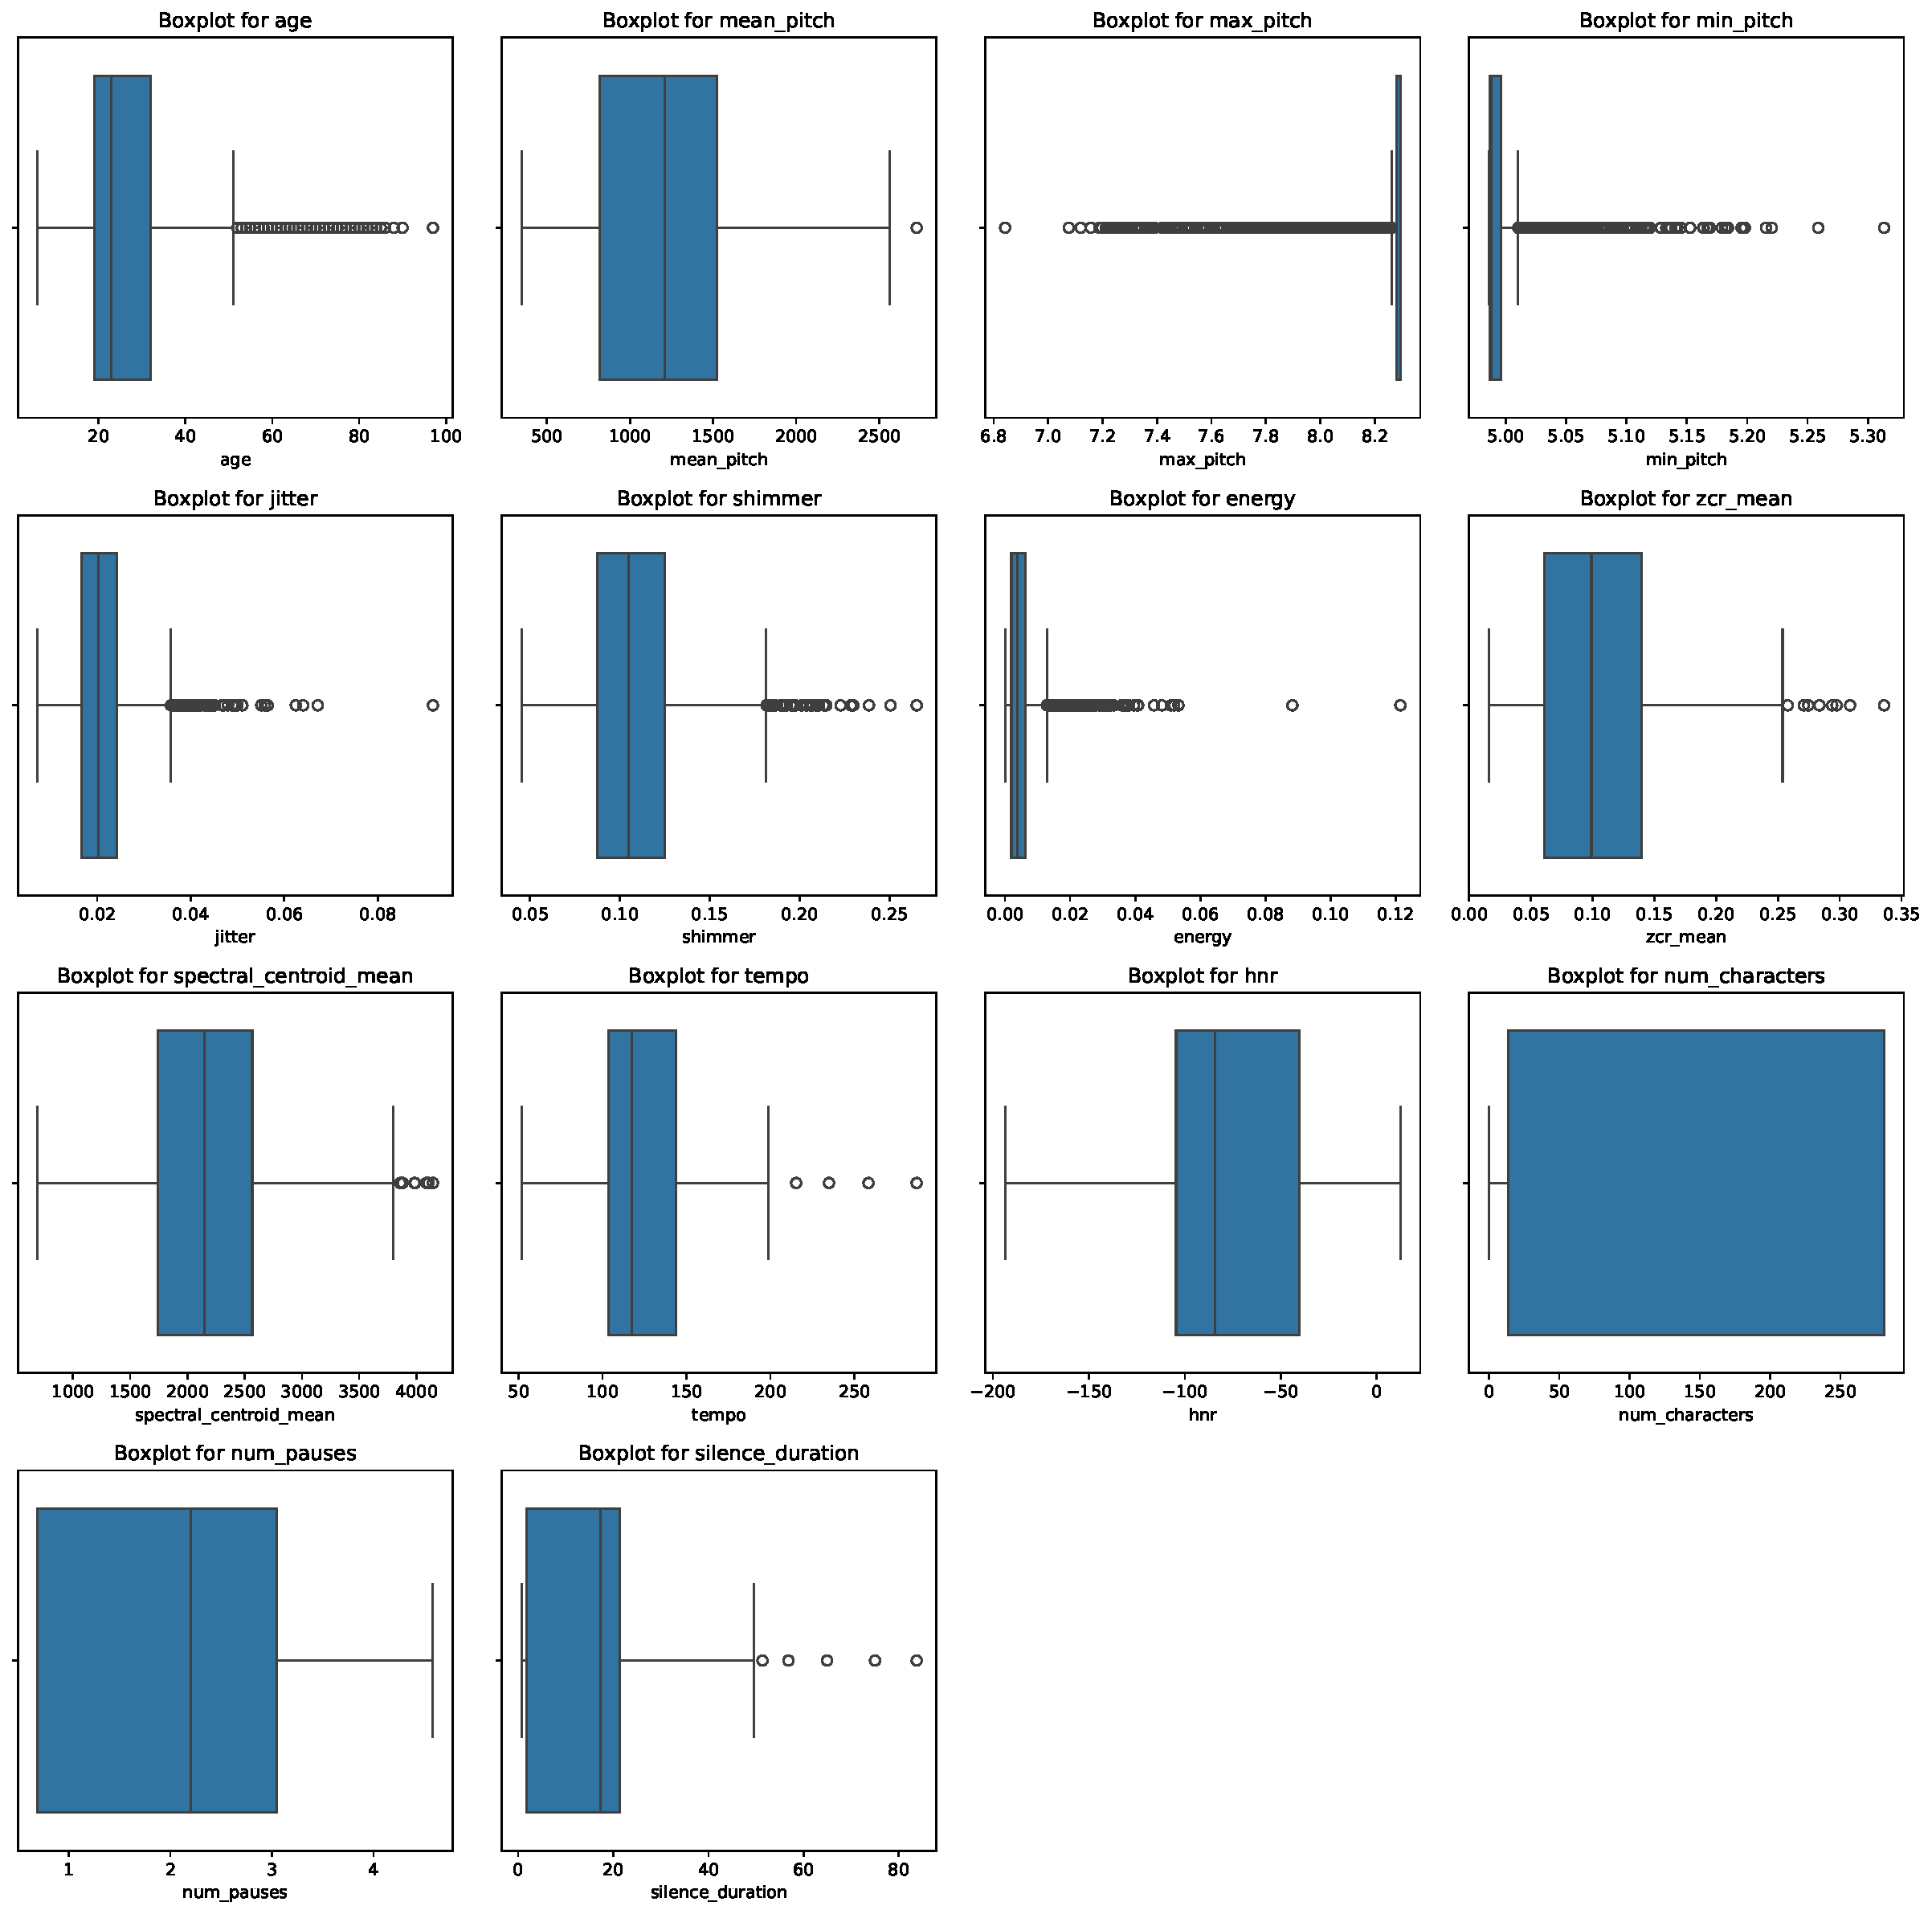
\includegraphics[width = 0.47\textwidth]{img/boxplot.pdf}
    \caption{boxplot of numerical features}
    \label{box}
\end{figure}

Then, we proceeded by standardizing the dataset. It is known that machine learning estimators may poorly perform if the data are not standardized because features with higher variance in space may dominate the objective function.
 
